\documentclass[12pt,a4paper,oneside]{report} %class

% encode foregin characters
\usepackage[T1]{fontenc}

% hungarian language
\PassOptionsToPackage{defaults=hu-min,classmod=unchanged}{magyar.ldf}
\usepackage{t1enc}
\usepackage[magyar]{babel}
\selectlanguage{magyar}
\usepackage[utf8]{inputenc}

\usepackage[table]{xcolor}

\usepackage{csquotes}

\usepackage{paralist}



% for esoteric file path
\usepackage{grffile}

% load pdf files
\usepackage{pdfpages}

% create neat tables
\usepackage{tikz}
\usetikzlibrary{matrix}
\usepackage{tabularx}
\setlength{\extrarowheight}{2pt}


\newcommand*{\fullref}[1]{\hyperref[{#1}]{\ref*{#1} \nameref*{#1}}} % One single link

% UML
%\usepackage{emp}
\usepackage[school,simplified]{pgf-umlcd}
\usetikzlibrary{calc}
\usetikzlibrary{positioning}
\usepackage{fullpage}

% monospae font

% images 
\usepackage{graphicx}
\graphicspath{ {./images/} }

% set margins
\addtolength{\oddsidemargin}{-1.2cm}
\addtolength{\evensidemargin}{-1.2cm}
\addtolength{\textwidth}{2.4cm}
\addtolength{\topmargin}{-1.5cm}
\addtolength{\textheight}{3cm}

% Figures right after text
\usepackage{float}

% set TOC depth
\setcounter{tocdepth}{4}

% remove red color for hyperref in TOC
\usepackage[unicode]{hyperref}
\hypersetup{
   pdfborderstyle={/S/U/W 2.5}% border style will be underline of width 1pt
}


% add bibtex
\usepackage[backend=biber]{biblatex}
\BiblatexHungarianWarningOff
\addbibresource{./mainbibliography.bib}

% compare table settings
%\setlength{\arrayrulewidth}{0.1mm}
\setlength{\tabcolsep}{18pt}
\renewcommand{\arraystretch}{1.6}

\newcolumntype{s}{>{\columncolor[HTML]{AAACED}} p{2.5cm}}





%top matter
\title{%
	
\includegraphics[scale=0.1]{logo_oe}\\
	ÓBUDAI EGYETEM\\
	Neumann János Informatikai kar\\
	Mérnök informatikus BSc\\
	\vfill
	\large \textbf{Vizuális, interaktív programozás oktató rendszer moduláris megvalósítása\\}
	\large Projektmunka dokumentáció
	\vfill
}
\author{Ráncsik Áron}
\date{\today}

\begin{document}

% 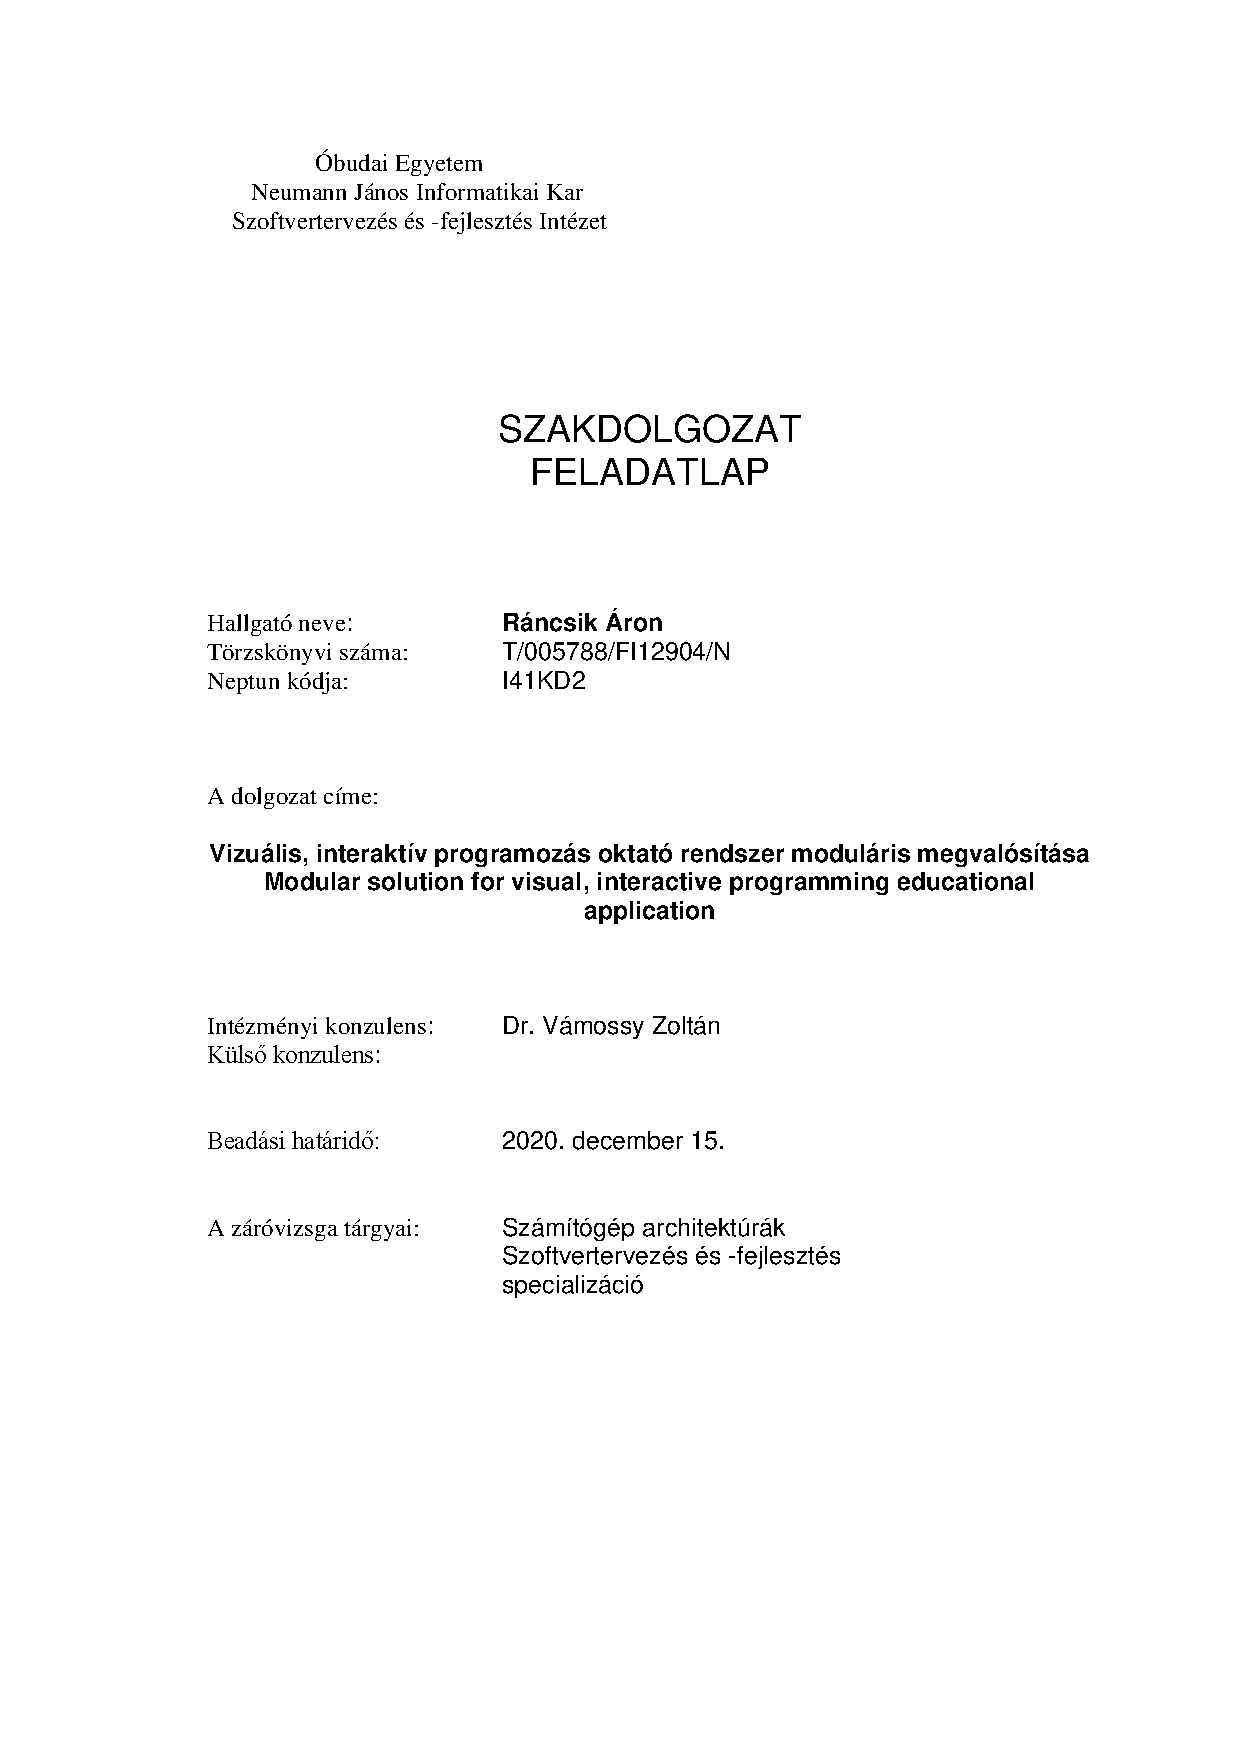
\includepdf[page={1,2}]{resources/feladatlap}
\pagenumbering{Alph}
\begin{titlepage}
%\maketitle
\thispagestyle{empty}
\end{titlepage}
\pagenumbering{arabic}

%\pagenumbering{Alph}
%\begin{abstract}
%	\thispagestyle{empty}
%	Your abstract goes here...
%	...
%\end{abstract}
\pagenumbering{arabic}

\tableofcontents

% Introductory chapters
\chapter{Bevezetés}
\par Először szeretném bemutatni azokat a célkitűzéseket, nem-funkcionális követelményeket, különböző elvárásaimat, melyek megvalósítását tervezem dolgozatomban. 
\par Fő célom, egy olyan rendszer elkészítése, melynek a segítségével, fiatal (10-16 éves) korosztály számára  lehet, elérhetővé, élvezetessé tenni a  programozást, algoritmizálást. Kedvcsináló módon,  szeretném az algoritmizálás tanulásra rávezetni a fiatalokat. Egy szokványos tanóra kereteit jóval túlhaladó igényeket kielégítő rendszer elkészítését tervezem.
\paragraph{További fontos követelmények, célok}
A fő célon túl további ötleteim, terveim vannak, ezeket részletezem itt.
\begin{enumerate}
	\item Nem egy létező programozási nyelv keretin belül szeretném  az algoritmizálás bemutatását megtenni. Ezzel szembeni követelményem, egy grafikus felület, \textit{GUI}, mellyel egyedi utasításokat teljesítő algoritmusokat lehet szerkeszteni, barátságos módon.
	\item Cél, hogy ne szokványos (logikai) feladatok elvégzésére készüljenek, a felhasználók által összerakott algoritmusok. Az előbb említett algoritmusokra, továbbiakban az ''ágens`` kifejezést használom. Az előbbi állítással szemben, azt szeretném, hogy az ágensek,  egymás elleni versengés, megmérettetés és játék, céljából készüljenek.
	\par Egy példán keresztül szemléltetve, azt szeretném, hogy egy egymás ellen játszható játékon belül, minden felhasználó egy számára kijelölt ''játékost`` irányíthasson az ágensével, és így az ágensek és a felhasználók is versengjenek, küzdjenek egymással. Az ilyen eszközöket használó oktatási formát, játékos oktatásnak  \cite{riar2020game}, vagy idegen szóval a \textit{gamification}-nek \cite{Deterding2011} nevezik. 
	\item Az ágensek küzdelmét, kiterjesztett valóságon keresztül is figyelemmel kísérhetővé szeretném tenni. Ennek a szemléltetésére is szeretnék példát írni. Tegyük fel, hogy  az ágensek küzdelme, egy kitüntetett környezetben, számítógépen történik, azon túl hogy az adott gép kijelzőjét kilehet vetíteni, a közdelem egy telefon és annak kamerája segítségével, az íróasztal lapjára is kiterjeszthető kell hogy legyen. Ezzel további jó hangulatot lehet teremteni.
	\item Az egymás ellen küzdő ágens programozáson túl, szeretném, ha a programozást biztosító grafikus felület, a da Vinci robotkar könnyű programozásra is használható legyen. Úgy gondolom, hogy a programozásoktatást egyik legszemléletesebb területe, a robotprogramozás. Továbbá, magas-szintű program utasítások biztosításának a segítségével könnyen, érthetően lehet szemléltetni a robotika és orvosinformatika területének szépségeit is, és a programozáson túl, az orvostudomány, robotika iránt is  lehetséges érdeklődést kelteni a fiatalokban.
\end{enumerate}

\newpage
\paragraph{A dolgozat áttekintése és kihívások bemutatása}
Most egy előretekintő és a dolgozatot valamelyest összefoglaló, vázlatot, szeretnék adni. A következő példa igyekszik bemutatni, hogy, hogyan gondoltam el, az egész rendszer használatát, működését, továbbá szeretném bemutatni, hogy a különböző kihívásokat az irodalom kutatás, mely részében tárgyalom részletesen.
\par A rendszer konkrét működését, felosztását, architektúráját a különböző alrészekben lehet megtekinteni itt: \fullref{munakterv}.

\subparagraph{Vázlatos működés felhasználó szempontjából}
\begin{enumerate}
	\item Egy felületen csatlakozik, megad egy egyedi azonosítót, nevét, esetleg regisztrálhat is.
	\item Hozzáfér a grafikus programozást nyújtó szerkesztői felülethez. Azt, hogy milyen lehetőségek vannak, ilyen grafikus programozó felület készítésére a: \fullref{vizuprogkor} résznél fogom tárgyalni.
	\item Attól függően, hogy da Vinci vagy játék programozási módban vagyunk, a felhasználó különböző egyedi utasításokat illeszthet össze ágenssé, például da Vinci esetén ''Fogd meg az 1. objektumot`` vagy játék módban ''Lépj jobbra`` , illetve alapvető ciklus és elágazás, utasításokat is tud használni.
	\item Van lehetősége helyi gépen történő tesztelésre. Mindenki futtathatja, tesztelheti saját eszközén is az elkészült ágensét.
	\item Miután mindenki összerakta az ágenseit, az oktató ezeket távolról összegyűjtheti és egy kijelölt gépen elindíthatja. Így például játék módban a küzdelem, valamilyen nagyobb kijelzőn  mindenki számára  megtekinthető.  Az előbbi lépések konkrét megvalósítási terve a későbbiekben bemutatott \fullref{felhkliens} különböző alrészeiben található.
	\item Da Vinci mód esetén az összegyűjtött ágensekből, oktatóknak van lehetősége egyet kiválasztva futtatnia a da Vinci roboton, vagy annak szimulációjában. A da Vinci robothoz történő kapcsolódási lehetőségek irodalomkutatása megtekinthető itt: \fullref{sec:davi}.
	\item Akár, mindenki telefonján elérhető, vagy egy erre szolgáló  eszközön, kiterjesztett valóságon keresztül is követhető az ágensek  küzdelme. A kiterjesztett valósággal kapcsolatos irodalom kutatás megtekinthető itt: \fullref{kitval}. Igyekeztem áttekinteni a kész megoldások listáját, továbbá utánajárni, a saját készítésű kiterjesztett valóság megvalósítás hátterének.
\end{enumerate}
 
%\paragraph{Algoritmus elmélet}
%Az algoritmus definiálása nehéz feladat, erre nem vállalkoznék, azt ki merem jelenteni, hogy azokat a feladatokat lehet algoritmizálni, melyek működése Turing-gép segítségével megvalósítható. A fiatalok számára az algoritmikus gondolkozást igyekszem szemléltetni. Az évek során több paradigma kialakult a programozásra, melyek inkább már az absztrakt gondolkozást részesítik előnyben. Úgy gondolom, hogy termesztésen ezeknek is helyük van az oktatásban, de az alapvető algoritmikus gondolkozásmód kialakításához nem szükségesek sőt, véleményem szerint hátráltatóak. A későbbikben részletezett vizuális programozó környezet vizsgálatakor, termesztésen alapvető elvárás volt részemről, hogy az adott megoldás ''Turing-teljes`` legyen. Bár a vizsgált megoldások többsége több, különböző paradigma eszközeit tartalmazza, ezeknek a tulajdonságoknak nem tulajdonítottam különösebb prioritást a vizsgálat során. A későbbiekben választott módszer, a strukturált programozási paradigmát támogatja.

\chapter{Módszertan}
\label{modtan}
A korában megfogalmazott célok elérése érdekében végzett, kutatómunkát részletezem itt.
Az elkészült alkalmazás működését is szeretném oktatási célokra felhasználni, ezért a megvalósítás során, olyan könyvtárakat igyekszem használni,  melyek forráskódja, működése szabadon elérhető. Amennyire lehetséges igyekszem az egyszerűbb megvalósítások irányában hajlani, értem ez alatt azt, hogy inkább olyan megoldások használatát preferálom, ami ''csak`` egy adott feladatra biztosít megoldást, de a használatához nem szükséges egy nagy, bonyolult rendszert használni. Az előbbi állításomból kifolyólag, például mellőzni igyekszem a különböző felhőszolgáltatások és zárt könyvtárak, valamint az ilyen komplett óriási kódbázisok, játékmotorok használatát.
\section{Vizuális programozási környezet}
\subsection{Alternatív megoldások vizuális programozásra}
\label{vizuprogkor}
Mivel a dolgozatban vizuális  programozást  is szeretnék biztosítani, ezért megvizsgálom milyen konkurens megoldások léteznek erre a célra. Az alábbiakban bemutatok és elemzek több kutatást, korábbi kész alkalmazásokat és programkönyvtárakat melyek mindegyike a vizuális blokk alapú programozásról szól.
\subsubsection{Scratch} 
\label{scratch}
Nagyon népszerű, oktatásban méltán közkedvelten használt teljes környezet \cite{maloney2010scratch, resnick2009scratch, ScratchUrl2019Jan}, mely vizuális programozást tesz lehetővé. Az alapvető célja, média alkalmazások mint például animáció, köszöntések, történet mesélés, zeneklip elkészítésének - folyamata közben megtanítani a programozást. Az egyedüli, intuitív tanulást is előnyben részesíti. Főleg kisebb 8-16 éves korosztály számára készült. 
\par Az elkészült program alapértelmezetten egy saját ``{színpad}'' környezetben futtatható. Esemény vezérelt programozást is lehetővé tesz, ebben az esetben, egyszerre fellépő konkurens utasítások között esetleges versenyhelyzetet kezeli, de nem minden esetben úgy ahogy azt elsőre a használó gondolná.  A programból \textit{broadcast} utasításokkal, saját parancsok, szkriptek végrehajtása lehetséges. A \textit{broadcast} utasítássokkal lehetséges a külvilággal történő kommunikáció is, de körülményes. Kiegészítőkkel bővíthető, de így sem lehet az alap működésre kiható szignifikáns módosításokat eszközölni.
\paragraph{Előnyei} 
\begin{compactitem}
	\item Szabadon elérhető, nyílt forráskódú.
	\item Kész megoldásról beszélve, sokkal kevesebb munka segítségével lehet használni.
	\item Egyedi működés \textit{broadcast} utasításokkal lehetséges.
	\item Az alap környezet többnyire magas szintű előre definiált utasításokban gazdag pl.: animációk
	\item Kezdők számára is egyszerűen érthető felület.
	\item Tapasztalatok alapján nagyon ismert az általános iskolások körében.
	\item Érthető, naprakész dokumentáció áll rendelkezésre
\end{compactitem}
\paragraph{Hátrányai} 
\begin{compactitem}
	\item A \textit{broadcast} utasításon kívül máshogy nem megoldható egyedi utasítás létrehozása.
	\item Az elkészült program csak a saját környezetén belül futtatható, nem lehetséges egyedi környezetben futtatni.
	\item Az elkészült program egyszerűen nem alakítható valódi programkóddá. (Van harmadik féltől származó kész megoldás)
	\item Monolitikus, bővítésre nézve többnyire zárt rendszer.
	\item Ugyan van webes felület, de saját oldalba nem ágyazható.
\end{compactitem}

\subsubsection{Snap} \label{snap}Új, még kevésbé  ismert, teljes megoldás \cite{harvey2013snap}, segítségével vizuálisan van lehetőségünk programozni. A \nameref{scratch}-el szemben több szabadságot biztosít a személyre szabhatóság tekintetében. Sokkal bonyolultabb problémák megoldására is alkalmas, az objektum orientált paradigmát is támogatja. A környezet kevésbé kezdőbarát. \textit{Url} utasításokkal webes  csatlakozó felületen keresztül tud fogadó és küldőként is könnyen kommunikálni a külvilággal. Érdekességként felhő alapú gépi tanulás szolgáltatásokhoz csatlakoztatva akár ``AI'' fejlesztésre is alkalmas \cite{kahn2018ai}. A párhuzamos ciklusokat időosztásos módszerrel futtatja párhuzamosan ``yield'' utasítások segítségével, de erre is igaz. hogy mindezt igyekszik elrejteni a felhasználók elől és nem igényel különösebb beavatkozást, az alapvető működéshez hozzá lehet szokni.
\paragraph{Előnyei} 
\begin{compactitem}
	\item Szabadon elérhető, nyílt forráskódú.
	\item Kész megoldásról beszélve, sokkal kevesebb munka segítségével lehet használni.
	\item Egyedi működés \textit{url} utasításokkal lehetséges. Sokkal kényelmesebben mint \nameref{scratch} esetén.
	\item Az alap környezet előre definiált utasításokban gazdag pl.: \textit{sprite}-ok vezérlése.
	\item Bonyolultabb problémák megoldására is alkalmas.
	\item Érthető, naprakész dokumentáció áll rendelkezésre
	\item Van webes felülete, de saját oldalba nem ágyazható.
	\item Egyedi blokkok létrehozását támogatja.
	\item Objektum orientált paradigmát támogatja
\end{compactitem}
\paragraph{Hátrányai} 
\begin{compactitem}
	\item Az elkészült program csak a saját környezetén belül futtatható, nem lehetséges egyedi környezetben futtatni.
	\item Az elkészült program nem alakítható valódi programkóddá.
	\item Nem biztosít felhasználható könyvárat, csak a projekt forrását felhasználva lehet egyedi alkalmazásokban használni.
	\item Jelenleg (\date{\today}) béta állapotban van.
	\item Monolitikus, bővítésre nézve többnyire zárt rendszer.
	\item A objektum orientáltság különböző megkötésekkel érhető el.
\end{compactitem}

\subsubsection{GP} Általános célú blokk alapú \cite{ohshima2015module} \cite{monig2015blocks} programozási nyelv. Egy valódi programozási nyelv, mely blokk és kód alapú programozási lehetőséggel is rendelkezik.  Sok alacsony szintű funkciók érhetőek el benne. Sokkal közelebb áll a valóságos programozáshoz a korábban említett lehetőségekhez képest, rendelkezik webes felülettel és a külvilággal internetes \textit{get}, \textit{put} utasítás lehetséges a kommunikáció egyedi rendszerekkel. Támogatja az objektum orientált paradigmát. Tartalmaz bonyolultabb adatszerkezeteket is.
\paragraph{Előnyei} 
\begin{compactitem}
	\item Kész megoldásról beszélve, sokkal kevesebb munka segítségével lehet használni.
	\item Egyedi működés \textit{get, put} utasításokkal lehetséges. \newline Sokkal kényelmesebben mint \nameref{scratch} esetén.
	\item Az alap környezet többnyire alacsony szintű előre definiált utasításokban gazdag pl. \textit{set pixel} utasítás blokk.
	\item Bonyolultabb problémák megoldására is alkalmas.
	\item Moduláris módon készült.
	\item Érthető, naprakész dokumentáció áll rendelkezésre.
\end{compactitem}
\paragraph{Hátrányai} 
\begin{compactitem}
	\item Az elkészült program csak a saját környezetén belül futtatható, nem lehetséges egyedi környezetben futtatni.
	\item Az elkészült program nem, vagy csak nehezen alakítható valódi programkóddá.
	\item Ugyan van webes felület, de saját oldalba hivatalosan nem ágyazható.
\end{compactitem}

\subsubsection{Alice} Interaktív 3D Animációs környezet \cite{cooper2000alice}. Az idézett kutatás által megfogalmazottan a  célja egy 3D-s környezet interaktív fejlesztése melyben szabadon lehet felfedezni az elkészült alkotást. Főleg szkript alapú, prototípus fejlesztő környezet. 
\paragraph{Előnyei} 
\begin{compactitem}
	\item Kész alkalmazás
	\item Adott 3D környezet
	\item Eseményvezérelt programozás tanítására is alkalmas
\end{compactitem}
\paragraph{Hátrányai} 
\begin{compactitem}
	\item Az elkészült program csak a saját környezetén belül futtatható, nem lehetséges egyedi környezetben futtatni.
	\item Nem vizuális egy sajátos egyedi szkriptnyelvvel rendelkezik.
	\item Az elkészült program nem alakítható valódi programkóddá.
	\item Nincs webes felülete, futtatható állományok telepítését igényli.
	\item Kissé régi, idejét múlt, már kevésbé támogatott.
\end{compactitem}

\subsubsection{Egyéb kész megoldások}
A fenti részben, a dolgozatommal legjobban összehasonlítható szempontok alapján fontosnak tartott kész megoldásokat mutattam be. Természetesen rengeteg egyéb kész alkalmazás létezik mely vizuális programozási lehetőséget biztosít. Felsorolás szintjén itt leírok pár szerintem említésre méltó alkalmazást. 
\begin{compactitem}
	\item Game Maker \cite{jenson2016exploring} 2D játék készítő, vizuális és saját szkriptnyelvvel is rendelkezik. A teljes verzió pénzbe kerül.
	\item Stencyl \cite{liu2014making} 2D Játék készítő alkalmazás melyben vizuálisan lehet programozni.
\end{compactitem}
A továbbiakban kész alkalmazások helyett, vizuális programozásra készült programkönyvtárak bemutatásával fogom folytatni a választható megoldások listáját.  
\subsubsection{Blockly}
\label{blocly}
Google által fejlesztett, vizuális programozást támogató programkönyvtár \cite{BlocklyUrl2020Feb} \cite{pasternak2017tips}. A vizuális megjelenésért felelős, nem egy programozási nyelv, csak egy vizuális leíró nyelv, mely könnyedén exportálható vallós programkóddá. Több létező programnyelv kódot lehet a vizuális környezetből generálni, többek között: JavaScript, Python, Lua, Dart nyelvű kódokat is. A Blockly könyvtárat sok kész alkalmazás használja a saját egyedi vizuális környezetének megvalósítására.
Például a korábban említett \nameref{scratch}, \nameref{snap} is használja vizuális könyvtárként, de az ezután részletezett \nameref{pxt} környezet is Blockly-t használ a vizuális megjelenítésre.
\paragraph{Előnyei} 
\begin{compactitem}
	\item Szabadon elérhető, nyílt forráskódú.
	\item Kezdők számára is egyszerűen érthető felület.
	\item Érthető, naprakész dokumentáció áll rendelkezésre.
	\item Programkönyvtár, könnyen bővíthető egyedi utasításokkal
	\item A program futtatási környezetére nincs megkötés.
	\item Nemzetközi. Több mint 40 (köztük magyar) nyelven elérhető.
	\item Bármilyen futtatási környezetbe könnyen integrálható.
	\item Rengeteg programkód generálható.
\end{compactitem}
\paragraph{Hátrányai} 
\begin{compactitem}
	\item Csak egy vizuális programozást támogató  ``drag \& dropp'' programkönyvtár.
	\item Viszonylag régi technológiákkal készült, nehézkes modern környezetben használni.
\end{compactitem}

\subsubsection{MakeCode (PXT)}
\label{pxt}
Microsoft által fejlesztett, összetett, vizuális programozói környezetet biztosító, nyílt forráskódú programkönyvtár \cite{seneviratne2019makecode}. A \nameref{blocly} könyvtárat felhasználja blokkalapú vizuális programozás biztosítására. A blokkalapú programozáson túl biztosít lehetőséget a szöveges programozásra is, egy beépített weboldalon futamítható fejlesztő környezetben. Abban különbözik a korábbi alternatív lehetőségektől, hogy egyben nyújt egy teljes fejlesztő környezetet, amihez könnyen hozzá lehet csatolni egy saját \textit{target} modult egyedi utasításokkal. A \cite{devine2018makecode} kutatás részletesen bemutatja, hogyan lehet használni beágyazott rendszerekhez.
\paragraph{Előnyei} 
\begin{compactitem}
	\item Szabadon elérhető, nyílt forráskódú.
	\item Kezdők számára is egyszerűen érthető felület.
	\item Érthető, naprakész dokumentáció áll rendelkezésre.
	\item Program könyvtár, könnyen bővíthető egyedi utasításokkal
	\item A program futtatási környezetére nincs erős megkötés.
\end{compactitem}
\paragraph{Hátrányai} 
\begin{compactitem}
	\item Integrálása korlátozott, alkalmazkodni kell a felépítéséhez, ettől eltérni nem lehetséges könnyen.
	\item Bétav verzióban van a fejlesztés.
\end{compactitem}

\subsection{Választott vizuális programozási környezet}
Kipróbáltam, teszteltem a legtöbb felsorolt megoldást, továbbá a korábbi elemzés összevetése  után a Blockly környezet használata mellet döntöttem.
A dolgozat igényeit nem lehet kész megoldásokkal pl. \nameref{scratch}, \nameref{snap} stb. kielégíteni, mert túlságosan zárt működésük nem teszik lehetővé, hogy egyedi környezethez lehessen programozni ezekben az alkalmazásokban.
A Blockly kellőképpen módosítható és könnyen egyedi környezetbe illeszthető, vizuális programozást biztosító programkönyvtár, mely megfelel a feladat részéről támasztott elvárásoknak, továbbá kellőképpen egyszerűen használható.


\section{Da Vinci}
\label{sec:davi}
A célok között szerepelt a da Vinci robot egyszerű vezérlése. 
Az elkövetkező részben, igyekszem körbejárni a lehetőségeket és elemezni előnyeit hátrányait, melyek segítségével lehet kapcsolódni a da Vinci rendszerhez. Az egyetemen egy 2010-ben bemutatott első generációs da Vinci classic rendszerhez van lehetőség hozzáférni, ezért ehhez készül az alkalmazás. A továbbiakban mindig erről a modellről lesz szó.
\subsection{Robot Operating System}
Annak érdekében, hogy a fejlesztés során, ne kelljen folyamatosan egy fizikai da Vinci rendszerrel dolgozni, egy olyan környezetre van szükség ami képes biztosítani da Vinci robotot virtuálisan. Több rendszer elérhető mely robot programozás vezérlő környezetet biztosít, csak felsorolás szintjén néhány \cite{BibEntry2020May, montemerlo2003perspectives}, azonban az egyik legkorábbi és legnépszerűbb lehetőség a Robot Operating System \cite{quigley2009ros} továbbiakban ROS. A ROS órási és növekvő közösséggel rendelkezik, \textit{de facto} standard az iparban és kutatásban. Dolgozatomban több szempont miatt is a legjobb választásnak a ROS rendszer bizonyult. Attól a hátrányától eltekintve, hogy nem multiplatform azaz csak Ubuntu GNU/Linux és annak is csak bizonyos verzióihoz támogatott hivatalosan, rengeteg előnnyel rendelkezik. Sok robotvezérléssel kapcsolatos alapfunkciót tartalmaz, amit így nem kell újból megírni, biztosít egy jól elszeparált keretet külön a kommunikációra és az üzleti logikára.
\paragraph{Előnyei} 
\begin{compactitem}
	\item Szabadon elérhető, nyílt forráskódú
	\item Kiforrót
	\item Népszerű
	\item Moduláris
	\item Kutatási célokhoz megfelelő
	\item Érthető, naprakész, jó dokumentáció áll rendelkezésre
\end{compactitem}
\paragraph{Hátrányai} 
\begin{compactitem}
	\item Nem multiplatform, csak Ubuntu GNU/Linux és annak is csak bizonyos verzióihoz elérhető
\end{compactitem}

\subsection{Da Vinci Research Kit}
\label{davinci}
A da Vinci Research Kit továbbiakban dVRK egy nyílt forráskódú rendszer, ami lehetővé teszi a Da Vinci robot karok programozását \cite{kazanzides2014open}. Gyakorlatilag ''firmware``-ként lehet rá tekinteni, ami képes meghajtani a robotkarokat.  A ROS rendszerhez kapcsolódik, könnyen lehetséges az utasításait használni egy ROS  modult biztosít használatra.  A célkitűzéseimhez képest viszonylag alacsony-szintű da Vinci robotkarvezérlő utasítások kiadására alkalmas.
Ennek a modulnak a segítségivel lehetséges a ROS rendszerrel da Vinci robotot vezérelni, továbbá virtuálisan szimulált robotkar létrehozása is lehetséges. mindenképp szükség van erre, amennyiben ROS rendszerhez szeretnénk kapcsolni da Vinci robotot. 
\subsection{iRob Surgical Subtask Automation Framework}
\label{irob}
Nagy D. Tamás és Haidegger Tamás által fejlesztett keretrendszer továbbiakban SAF \cite{irobsaf2019}.
Alapvetően arra a célra készült, hogy részleges automatizáció segítségével levegye a sebészekről a kognitív terhelést. Részfolyamatok automatizálását teszi lehetővé a keretrendszer. A ROS rendszerben elérhető modulokat biztosít, a dVRK rendszerre épül. Használata során felépít egy hierarchikus modul rendszert, melynek a legmagasabb szintjén magas-szintű utasítások kiadása lehetséges. Számomra a céloknak tökéletesen megfelelő.
\paragraph{Előnyei} 
\begin{compactitem}
	\item Szabadon elérhető, nyílt forráskódú
	\item Moduláris
	\item Alkalmas Kutatási célokhoz
	\item Érthető, naprakész, jó dokumentáció áll rendelkezésre
\end{compactitem}
\paragraph{Hátrányai} 
\begin{compactitem}
	\item Jelenleg fejlesztés alatt áll.
\end{compactitem}


\section{Kiterjesztett valóság}
\label{kitvalo}
A célok között szerepelt egy olyan funkció, melynek a segítségével lehetséges kiterjesztett valóság segítésével követni az ágensek küzdelmét. Itt szeretném részletezni a hasonló megoldásokat, azokból levont következtetéseket.
A \cite{azuma2001recent} kutatásból idézve  kiterjesztett valóságot a következő módon definiálhatjuk. Az a rendszer, ami a következőket teljesíti:
\begin{compactitem}
	\item Kombinálja a valós és virtuális objektumokat a valós környezetben.
	\item Azonnal fut, és valós időben.
	\item Egymáshoz rögzíti (igazítja) a valós és virtuális objektumokat.
\end{compactitem}
Továbbikban az AR rövidítést fogom használni. 
Virtuális objektumokat szeretnénk elhelyezni a kamera képen úgy, hogy azok mozgása a kamera 3D mozgásához igazodjon. 
\par Több létező megoldás van AR elkészítéséhez, ezen megoldások összehasonlításáról lesz itt szó.
A legtöbb esetben nagyobb gyártók szolgáltatásaként lehetséges ilyen alkalmazásokat használni.
\subsection{Alternatív kiterjesztett valóság megoldások}
\label{kitval}
\subsubsection{Unity}
Unity Technologies által fejlesztet játékmotor. 2D és 3D számítógépes játékok elkészítésre alkalmas. Napjaink egyik, ha nem a legnépszerűbb játék fejlesztő motorja \cite{haas2014history}.
Rengeteg játékkészítéssel kapcsolatos funkciót biztosít. AR megvalósításához rendelkezik saját megoldással. Itt \cite{kim2014using} egy példa látható arra, hogyan lehetséges a Unity beépített AR megoldását használni és milyen előnyök származnak ebből, illetve a Unity használatából. Az előbbi hivatkozott példában láthatjuk, hogy rengeteg kényelmi funkcióval rendelkezik, melyek használata, csupán kiterjesztett valóság rendszerekben, játékmotor nélkül, sokkal körülményesebb.  További előnye, hogy a Unity rendszerrel készült alkalmazások az összes ma használatos platformra fordíthatóak. 
\paragraph{Előnyei} 
\begin{compactitem}
	\item Ingyenesen használható
	\item Érthető, naprakész, jó dokumentáció áll rendelkezésre
	\item Használata könnyű
\end{compactitem}
\paragraph{Hátrányai} 
\begin{compactitem}
	\item Nagyon nagy függőség
	\item Kifejezetten játék fejlesztésre van, rengeteg extra funkcióval rendelkezik
	\item Nem lehetséges csak modulként használni
	\item Feltétlen alkalmazkodni kell a használatához
	\item Nem nyílt a forráskódja
\end{compactitem}
\paragraph{Konklúzió}
Úgy gondolom, hogy túlságosan nagy erőforrás és munka pazarlás lenne Unity-t csak kiterjesztett valóság elkészítésére használni. Egyáltalán nem vagy csak nagyon sok plusz munka árán lehetne alkalmazásba integrálni, inkább az alkalmazást kellene a Unity-be integrálni használata esetén.

\subsubsection{Unreal Engine}
Egy szoftver amely valósidejű 3D grafika készítésére készítettek \cite{unrealengine}. Szűkebb értelemben játékmotornak is lehet  nevezni. Szintén rendelkezik saját megoldással Virtuális valóság (VR), AR és kevert valóság (MR) számára is.
\paragraph{Konklúzió} Többnyire ugyanazok igazak rá mint a Unity-re ezért külön nem tárgyalom. A fejlesztést marginálisan meghatározná, a motor használatához kellene alkalmazkodni.
\subsubsection{Mobil megoldások}
\paragraph{iOS ARKit}
Az ARKit segítségével, Apple iOS platformra lehetséges AR alkalmazást készíteni \cite{arkit}. A korábban említett különböző maga-szintű megoldások pl. Unity ezt a rendszert is használja, ha iOS platformra készítünk projektet. Egy AR alkalmazás számára szükséges összes funkciót megvalósítja, pl. a telefon kamera pozíció becslését, virtuális objektumok elhelyezését. Természetesen mint mobil megoldás, a telefon kameráját illetve szenzorrendrendszerét használja a működéshez.
\paragraph{ARCore}
Hasonlóan az ARKite-hez, az ARCore a modern Android operációs rendszerrel rendelkező telefonokon elérhető kiterjesztett valóságot biztosító API \cite{arcore}.
\paragraph{Konklúzió}
Az előbb említett megoldások használatához Andoid vagy iOS alkalmazás készítése szükséges. A legtöbb játékmotor is ezeket a megoldásokat használja mobil platformokon. Ezeknek a rendszereknek a teljes műkése rejtett, egy API-t biztosítanak melyen keresztül lehetséges használni, ugyan az API-n keresztül minden kínált funkció elérhető ,a működéshez ezen túl nem lehet hozzáférni. Ezek a megoldások jól működnek, de egyedi igényeket nem lehetséges velük kiszolgálni. A működésüket nem lehet megismerni, továbbá zárt forráskódú rendszerek. Ezeket figyelembe véve, számomra nem megfelelőek.
\subsubsection{Egyéb kész megoldások}
Itt olyan megoldásokat említek, melyeket kész alkalmazásként vagy könyvtárként lehetséges használni. Felsorolás szintjén a Vuforia \cite{vuforia}, Wikitude \cite{wikitude}.
Ezekről általánosan elmondható, hogy használatuk részben vagy teljesen nem ingyenes. Igyekeznek saját komplett felhőszolgáltatást kényszeríteni a használathoz. Forráskódjuk ezeknek is zárt. Használatukhoz a biztosított API-t kell használni egyedi megoldások megvalósítása ezekkel is körülményes.  A felsorolt hátrányok miatt számomra alapvetően nem alkalmasak használatra.
Az EasyAR \cite{ezar} és Kudan \cite{kudan} rendszerek használata bizonyos feltételek mellet ingyenes, de forrásuk továbbra is zárt. Többnyire ezekre is igazak a  fizetősekre felsorolt hátrányok.

\subsubsection{Egyedi megoldás}
Egy jó lehetőség lehet, saját kiterjesztett valóság megvalósítása, ingyenes program könyvtárak segítségével.
Azt értem az ilyen megoldás alatt, hogy a készítés során alacsonyabb-szintű gépi látás szintjén, egy saját kiterjesztett valóság szolgáltatást építünk. Egy ilyen megoldásnak több nehezebb feladatot kell tudni megoldania. Ilyen esetben a kiterjesztett valóság elkészítse a feladat, nem pedig egy AR szolgáltatás használata. Elkészítése a korábbiaknál nagyobb kihívást jelent. Az elérhető ''kész`` alkalmazások, könyvtárak komplett fejlesztő csapatok által, több év óta folyamatosan fejlesztés alatt vannak. Így teljesítmény szempontjából ezekkel szemben felvenni a versenyt szerintem lehetetlen, viszont modularitás és megérthetőség szempontjából úgy gondolom, hogy van értelme megpróbálni. A különböző megvalósítási lehetőségek megértése és adott feladathoz történő választása továbbra is egy előny, mert nem feltétlen kell általános megoldást készíteni.

\par Az egyik legnépszerűbb és  legjobban elterjedt gépi látással kapcsolatos programkönyvtár az eredetileg Intel által fejlesztett,  majd később nyílt forráskódú közösség által, a mai napig is folytatott OpenCV \cite{opencv_library}.
\subsection{Választott módszer}
Számomra fontos volt, hogy az AR rendszer átlátható kegyen, nem csak egy használható, de a működését megismerhető rendszert szeretnék használni. Korábban már többször említettem, hogy különböző játékmotorok használatát elvetettem, mert túlságosan alkalmazkodni kellene hozzá. 
\par A felsorolt (többnyire) zárt könyvtárak, használata sem biztosítja a megfelelő szabadságot, továbbá előnytelennek találtam azt, hogy forrásuk zárt.


\begin{figure}[H]
	\centering
	\begin{tabular}{s|p{3.5cm}|p{3.5cm}|p{3.5cm} }
	%\hline
	%\rowcolor{lightgray} \multicolumn{3}{|c|}{Country List} \\
	%\hline
	& Játékmotorok &(Részben) fizetős könyvtárak &  Egyedi megoldás \\
	\hline
	Forráskód & Zárt & Zárt & Nyílt \\
	%\rowcolor{gray}
	AR Sebesség & Jól optimalizált & Jól optimalizált & A fejlesztő feladata az optimalizáció \\
	Egyedi igények   & A maga játékmotor kínál rengeteg lehetőséget, hozzáköt a motorhoz & Saját ökoszisztémát nyújt, vagy korlátozottak a lehetőségek   & Teljes mértékben lehetőségünk van egyedi igények megvalósításra  \\
	Ár & Bizonyos feltételek mellet ingyenes & Bizonyos feltételek mellet ingyenes & Ingyenes\\
% \cellcolor[HTML]{AA0044}

	%\hline
	\end{tabular}
	\caption{Főbb AR megközelítési lehetőségek összehasonlítása}
\end{figure}

A különböző megoldásokat összehasonlítva, a saját AR megoldás megvalósítása mellet döntöttem. Fő indokom, egy olyan rendszer készítése, melynek a működése megérthető ennélfogva, amennyire lehetséges nem támaszkodik fekete-dobozokra.

\section{Saját AR készítéshez szükséges irodalomkutatás}
Annak érdekében, hogy saját AR rendszert készítsek, igyekeztem utána járni a lehetséges módszereknek, fogalmaknak.
Alapvetően abból indultam ki, hogy egy átlagos telefon kameraképeivel működjön a rendszer, így reális minőségű képekkel tudok dolgozni.
\subsection{Kamera kalibráció}
Kalibrált képen a valóságban egyenes szakaszok a képeken is így fognak megjelenni. Egy kamera rendelkezik külső és belső tulajdonságokkal. 
\paragraph{Külső tulajdonság} Így nevezzük, a 3D pozíció és  orientáció együttesét. Az előbb említett összetett  tulajdonság különösebb bizonyítás nélkül belátható, hogy egy transzformációs mátrix segítségével leírható.
\paragraph{Belső tulajdonság} 
Összetett tulajdonság mátrixban tárolva. A kamera középpontjának koordinátáit, a pixelek méreteit tartalmazza.  A kamerák képei nem tökéletesek. Tangenciális torzulás lehetséges az objektív miatt, ezt hívják halszem hatásnak is, ennek a korrigálását teszi lehetővé ezen tulajdonságok pontos meghatározása. 
\par  A kamera külső és belső paramétereinek megismerése érdekében a kamerakalibráció egy szükséges lépés a 3D gépi látáshoz. Itt \cite{zhang1999flexible} láthatunk, egy  napjainkban is elterjedt módszer működését.
\paragraph{A bemutatott kalibráció előnyei} 
\begin{compactitem}
	\item Nem igényel különösebben drága felszelést. 
	\item A folyamat könnyen kivitelezhető a kamera, mintázat szabad kézzel tartható 
	\item Pontosabb mint, az automatikus kalibrációs módszerek.
\end{compactitem}

\subsection{Képpontok egymásnak megfeleltetése}
Egy digitális képen alapvetően színek, fényességértékek sokaságaként tárolunk, ebből szeretnénk egy adott pontot megnevezni. A következő megközelítéseket vizsgáltam meg ennek érdekében. Egyszerűbb megközelítés, a klasszikusnak számító Multiple View Geometry című könyvben is találunk \cite[ó.~140]{hartley2003multiple}, melyben példaképp RANSAC \cite{derpanis2010overview} algoritmus segítségével, közelít optimális képpont megfeleltetést. Legegyszerűbben szerintem ezen a példán érthető meg.

\paragraph{Jellemző pontok keresése}
Az úgy nevezett, \textit{wide baseline stereo} megközelítésbe tartozik.
Bizonyos jellemzők \textit{feature} alapján lehetséges jellemezni képen egy pontot. Az a cél, hogy az adott karakterisztika, tulajdonság amivel jellemeztünk egy pontot, folyamatosan minél tovább, megmaradjon az egymás utáni képeken. Így az adott ''egyedi`` pont, több képen is beazonosítható. A jellemzőt előállító algoritmust \textins{feature descriptor}-nak hívja szakirodalom. Erről részletesebben fogok foglalkozni a következő bekezdésben.

\paragraph{Jellemző leírók}
Egy képből jellegzetes, többnyire nagy lokális kontrasztú pontokat jelölünk ki. Ezeket a pontokat fényviszony változása mellet, illetve átméretezett és átforgatott képen is szeretnénk megtalálni, ez utóbbit hívják méretezés és forgatás invarianciának.
\begin{figure}[H]
	\centering
	\begin{tabular}{s|p{3.5cm}|p{3.5cm}|p{3.5cm} }
		%\hline
		%\rowcolor{lightgray} \multicolumn{3}{|c|}{Country List} \\
		%\hline
		& SIFT \cite{lowe2004distinctive} & SURF \cite{bay2006surf} &  ORB \cite{rublee2011orb} \\
		\hline
		Ingyenes? & Nem & Nem & Igen \\
		Méret invarián? & Igen & Igen & Igen \\
		Forgatás invariáns? & Igen & Igen & Nem \\
		Elterjedtség & Mára kevésbé népszerű & Népszerű & Népszerű \\
		Egyéb tulajdonság 
		& Képes a pontról 8 irányban gradiens jellemzők alapján beazonosítást végezni.
		Minden talált ponthoz egy orientációt is meghatároz. 
		& A SIFT gyorsított változat., Kicsit pontatlanabb, de sokkal gyorsabb. Jól párhuzamosítható algoritmus. Közelítő módszerekkel számol, a gyorsaság édenkében 
		& Ingyenes alternatíva a SIFT és SURF algoritmusokra. Több módszer kombinációjaként született meg.\\
	
		%\hline
	\end{tabular}
	\caption{Jellemző leírók összehasonlítása}
\end{figure}


\paragraph{Optikai-folyam}
\textit{Optical Flow} (OF), \textit{Small deformation} kategóriába lehet sorolni, mely alap feltételezésében eltér a korábban említett \textit{wide baseline stereo} megközelítéstől. Az alap feltételezés, hogy nagyon kicsi két képkocka között a különbség, továbbá egy adott sugarú pixel környezet, nem feltétlen ugyanolyan, de hasonló  mozgást végez. A teljes mozgás \textit{smooth}, sima, nincsenek olyan pixelek amik a környezetüktől nagyon külön utat járnak.  A modell ellentétben a jellemzőpont keresésessel,  \textit{dense} sűrű ábrázolására alkalmasak. Kötelező megemlítenem a Lucas-Kanade \cite{lucas1981iterative} és Horn-Schunck \cite{horn1981determining} egyszerre, igen korán 1981-ben bemutatott kutatását. Horn módszere a az összes pixelhez  mozgás vektort rendel, ezért a korai időszakban nem volt valósidejű, de mára már annak lehet tekinteni. Kanade megoldása viszont, könnyebben megérthető. Ma már alap algoritmusnak, annyira közkedvelt és alapvető,  hogy videokártyák minta kódja között is lehet találkozni a különböző implementációkkal.
 

\subsection{Kamera mozgásának rekonstrukciója}
Miután ismerjük a kamera tulajdonságait a képekkel torzítás mentesen tudunk a továbbiakban dolgozni.
A kamera mozgásának meghatározása a kamerával készült képekből. A videó feldolgozása során, szeretnénk minden képhez, egy merev-test mozgást meghatározni, melyre igaz, hogy a virtuális objektumra történő alkalmazás esetén a tanformáció után az objektum a kamera képen, megfelelő szögbe és pozícióba kerül az objektum. Az első kép esetén természetesen külön kell dönteni a virtuális objektum elhelyezkedéséről.

\subsubsection{Simultaneous Localisation and Mapping}
Meg kell különböztetni az ismert és ismeretlen \textit{scene} ''jelenet``-ben történő kamera \textit{tracking} ''követés``-t. Ismeretlen jelenet esetén, egy lehetséges kidolgozott megközelítés a ''Simultaneous Localisation and Mapping`` (SLAM). Egy módszer arra, hogy a kialakított modell, \textit{structure} és kapott kép információk alapján lehetőleg minél pontosabban szeretnénk a kamera merev-test mozgását meghatározni.
Az egyik nagy előrehaladás a 2003-ban bemutatott sokat hivatkozott valósidejű megvalósítás \cite{davison2003real}. A megoldás egy darab kamerát használt, \textit{monocular} ezt SLAM-nek szokás nevezni. 
Az ötlet a Kálmán szűrőn alapszik \cite{welch1995introduction}, mely a egy optimális becslő algoritmus. Egy modell állapotából és tapasztalat által szerzett zajos állapotból igyekszik optimális állapotot meghatározni. Ennek egy továbbfejlesztett megoldására latunk példát itt \cite{klein2008improving} mely a modellt magasabb szintű részekkel bővítette ki. A SLAM módszerekről elmondható, hogy legtöbb esetben a jellemző képpontok keresését és azok egymásnak való megfeleltetésének módszereket használnak, de optikai-folyam módszer alapján is működhetnek. 
Robotika területén, gyakran alkalmazzák, legtöbb specifikus programkönyvtár több variánsát támogatja.

\subsection{Saját AR, jelölő keresésén alapuló módszerrel}
Az eddigiektől egészen eltérően megközelítés. A kamera mozgásának meghatározása helyett, egy előre ismert \textit{marker}, ''jelölő``  keresése a cél. 

Egy előre kiszámolt hasítótáblázatból keres jelölőket a képeken. Fontos, hogy a jelölők konkrét fizikai méretének az ismeret is szükséges. Bináris négyzet alakú jelölőket keres. 
A \cite{garrido2014automatic} munkában részletesen leírják a jelölők detektálásának működését. Nagy vonalakban a következőképpen működik. 
\begin{enumerate}
	\item Szűrést véges négyzetnek tűnő alakzatokra, ezeket a jelölteknek hívjuk. Itt érdemes megemlíteni, hogy a keresett négyzetek tetszőlegesen elforgatva lehetnek a képeken.
	\item  Miután a jelöltek megvannak a tartalmukat bizonyos szabályossági tesztnek, idegenszóval a kijelölt négyzet belső tartalom kodifikációját kell ellenőrizni. Magyarán ellenőrizzük, hogy megfelel-e bizonyos szabályoknak, pl. mivel a jelölők mind fekete sávval vannak körbe véve, ezért lehet vizsgálni hogy a konkáv tulajdonságnak megfelelnek-e fekete sávok, vagy egyéb komplexebb tulajdonságot.
	\item Az elkészült modul, élő kamera folyamon próbál keresni egy előre megadott jelölő listákból minél többet, majd megjeleníti a 3D-s elhelyezkedését a talált jelölőknek.
\end{enumerate}
egy    Jelző beazonosításhoz szükség van kalibrált kamerára, magyarán ismerni kell a kamera és objektív torzulás mátrixokra, mert a torzítást ki kell korrigálni a keresés elött. Ezt a feladatot a OpenCV Aruco könyvtár segítségével oldottam meg.  A jelölő detektálást a könyvtár végzi. Az eredmény 6 jelölő alapú póz meghatározás ábrán is látható, a módszer valós idejű gyors, 

\paragraph{Összehasonlítás a korábbi ötlettel}
A megvalósítása sokkal kisebb számítás igénnyel rendelkezik.

\begin{figure}[H]
	\centering
	\begin{tabular}{s|p{5.5cm}|p{5.5cm} }
		%\hline
		%\rowcolor{lightgray} \multicolumn{3}{|c|}{Country List} \\
		%\hline
		& AR kamera pozíció rekonstrukcióval &  AR jelölő kereséssel \\
		\hline
		Kamera kalibráció & Szükséges & Szükséges \\
		Erőforrásigény & Magas & Közepes \\
		Használatához szükséges eszközök & Kamera & Kamera, jelölő \\
		Komplexitás & Bonyolult & Kevésbé bonyolult \\
		Előnyök, hátrányok 
		& Jól tűri a hibákat, viszont jelölő nélkül nem használható. 
		& Robusztusabb rendszer, előfordulhat drift jelenség.
		
		%\hline
	\end{tabular}
	\caption{Saját AR alapvető ötleteinek összehasonlítása}
\end{figure}


\subsection{Saját AR Konklúzió}
Az előbb tárgyalt elméleti módszerek, legtöbbjének legalább alapvető ismeretére, de adott esetben a teljes  működésével tisztában kell lenni, saját AR készítése során. Előreláthatólag nem lesz könnyű feladat megvalósítani. Főleg a futásidőre történő optimalizáció szempontjából sokkal rosszabb helyzetből indul, mint nagy gyártók által elkészült alternatívák. Mérlegelve a feladat nagyságát és értelmét, arra döntésre jutottam, hogy ezek ellenére is saját AR rendszer elkészítésébe kezdek. Úgy gondolom, hogy megéri ezen a területen kutatni, és egy egyszerűbb, de teljesen igényeknek megfelelő AR alkalmazást készíteni, ha más nem a elkészítés során szerzett új ismeretek miatt is.

\chapter{Részletes munkaterv}
\label{munakterv}
\section{Nevezéktan}
\paragraph{Fiatal} Azok a felhasználók, akik a célcsoportjai ennek az alkalmazásnak.
\paragraph{Oktató} Azok a felhasználók, akik a fiatalokat koordinálják, segítik.

\section{Felosztás}
A dolgozat méretére való tekintettel, a következő fogalmak bevezetésével felosztom a dolgozatot.
\paragraph{Rendszer}
''Rendszer``-ként fogok hivatkozni a teljes elkészült megoldásra.
\paragraph{Alkalmazások}
A rendszeren belül külön ''alkalmazásokra`` osztom a különálló, megoldandó feladatokat, melyek egymással Ethernet hálózaton vagy interneten kommunikálnak.
A következő alkalmazásokra és a hozzájuk  tartozó feladatokra bontottam a rendszert.
\begin{enumerate}
	\item Felhasználói kliens alkalmazás.
	\par Fő feladata, biztosítani: 
	\begin{compactitem}
		\item Grafikus programozási felületet
		\item Oktatók számára szükséges kezelőfelületet
		\item Közdelem megjelenítését
	\end{compactitem}
	\par További feladat:
	\begin{compactitem}
		\item Oktatói gépről, játék állapot adatok küldése a kiterjesztett valóság megjelenítő számára.
		\item Oktatói gépről, kapcsolat kiépítése és utasítások küldése a ROS WebSocket szerviz alkalmazás felé.
	\end{compactitem}

	
	\item Felhasználói szerver alkalmazás.
	\par Fő feladatai:
	\begin{compactitem}
		\item Autentikáció
		\item Fiatalok ágenseinek tárolása 
		\item Az ágensek eljuttatása az oktatói gépre.
	\end{compactitem}

	\item AR alkalmazás
	\par Fő feladata: Folyamatosan beérkező adatok 3D megjelenítése a kamera mozgásához igazítva.
	\par További feladat: kamerakalibráció elvégzése.

	\item da Vinci ROS környezet. Azon ROS modulok összessége, melyek szükségesek a da Vinci, ROS keretrendszerbe történő csatlakoztatásához illetve a szimulációhoz.
	
	\item ROS WebShocket szerviz alkalmazás
	\par Mediátor feladata van. Az oktatói számítógépről jövő utasítás, eljuttatja  a da Vinci ROS környezet megfelelő moduljának, valamint a választ továbbítja az oktató gépre.
\end{enumerate}

\subparagraph{Modulok}
Az alkalmazások belül, modulokból épülnek fel a részfeladatok megoldása mentén, egyszerű esetben egy osztály egy modult reprezentál, de vannak ennél összetettebb esetek is. Egy modul akár több másik modulra épülhet.

\subparagraph{Layout}
Főleg a rendszer \textit{front-end} részénél van értelme ennek újabb absztrakt csoportnak a bevezetésére, több különböző modul összerakásával készíthetünk egy ilyen felületet, melyen keresztül egy adott feladatot lehet ellátni, a modulok több \textit{layout}-ban is újrahasználhatóak, így igyekszem elkerülni a duplikációkat.


\section{Alkalmazásokhoz választott alapvető technológiák}
A teljes fejlesztés alapvetően GNU/Linux operációs rendszer alól történik. Több éve használom, és minden szempontból jobb számomra mint a többi konkurens OS.
\par Első döntésem az volt, hogy a felhasználói alkalmazásokat, webes technológiák segítségével fogom elkészíteni. Böngészőből futtatható lesz  az alkalmazás azon része, mely a felhasználókkal tartja a kapcsolatot. Így gyakorlatilag a platform különbséggel alkalmatosos problémák megszűnnek, manapság mindenhol fut a böngésző. A konkrét webes technológiát később részletezem. 
\par Az AR alkalmazás C++ és OpenCV segítségével fog elkészülni. C++ a sebesség, optimalizáció és népszerűsége szempontjából egy jó választás. A nehézkes szintaktikája, viszont megnehezíti a használatát. Korábban már említettem az OpenCV pozitív tulajdonságait, gyakorlatilag \textit{de facto} sztenderd gépi látással kapcsolatos programkönyvtár. 
\par A da Vinci rendszerhez történő kapcsolathoz szintén C++ nyelvet fogok, ahsonló okok miatt elletve már választásom itt nem is lenne. Továbbá a ROS  programkönyvtárat fogom még használni.  A ROS ról is elmondható, hogy robotika területén \textit{de facto} sztenderd. A ROS környezethez készült, dVRK és az ezen alapuló SAF könyvtárak használatára is szükségem lesz, a magas-szintű da Vinci utasítások kiadására. 

\section{Alkalmazások közötti kapcsolatok}
Korábban említésre került, hogy az alkalmazások Ethernet hálózaton, akár interneten keresztül kommunikálnak. A \ref{fig:kapcs} ábrán, a rendszer felépítésének terve és alkalmazások között közötti kommunikációs kapcsolatok láthatóak.
\begin{figure}[h]
	\label{fig:kapcs}
	\centering
	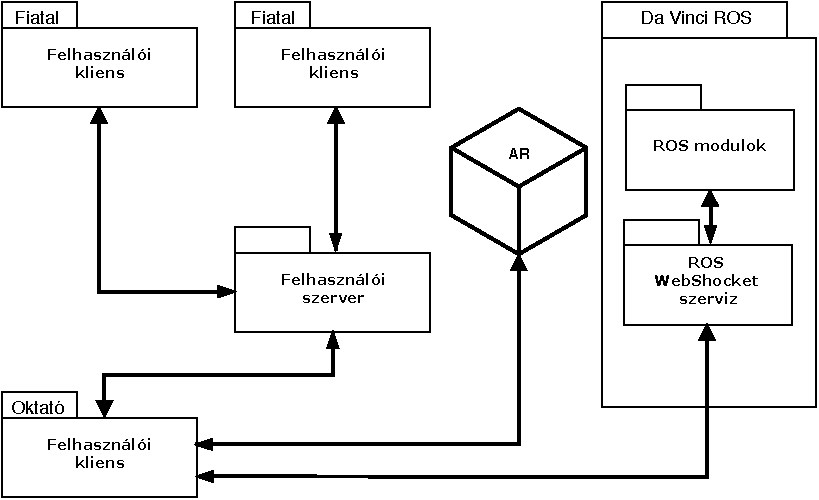
\includegraphics[width=0.75\textwidth]{dias/alkalmazas_kapcsolatok}
	\caption{Alkalmazások közötti kapcsolatok}
\end{figure}

\section{Alkalmazások tervezett felépítése}
Az egyes alkalmazások tervezésének részletei a következőkben találhatóak.
\subsection{Felhasználói szerver alkalmazás}
Korábban a webalkalmazás mellet döntöttem a felhasználói alkalmazásokkal kapcsolatban. Webes technológiákból rengeteg létezik, jobbnál-jobb újításokkal, azonban a felhasználói szerver nem annyira kulcsfontosságú része az alkalmazásnak. Gyakorlatilag bármilyen értelmes technológiával elkészülhetne, olyan kevés funkcióra lesz szükségem, hogy különösebb kutatás nélkül kiválasztottam az egyik kedvencemet a NodeJS-t.
Napjainkban továbbra is töretlenül népszerű technológia a NodeJS. Nem kifejezetten bonyolult webvállalkozásokhoz a használata kényelmes. Vertikálisan könnyen skálázható. Rengeteg elérhető programkönyvtár miatt pedig nagyon gyorsan lehetséges benne fejleszteni.
Az objektum orientált paradigma kényelmes támogatása céljából TypeScript nyelven tervezek írni. Express és WebShocket.io és egyéb csomagok segítségével egy egyszerű, minimális szervert szeretnék készíteni.
\subsubsection{Felhasználói szerver külső funkciók}
\begin{compactitem}
	\item Regisztráció / Autentikáció
	\item Ágens mentése / betöltése
	\item Ágensek begyűjtése
	\item Begyűjtött ágensek kiküldése oktató felé
	\item Felhasználók online állapotának nyilvántartása.
	\item Összes online felhasználó lekérése
\end{compactitem}
\subsubsection{Fiatal felhasználók tárolt adatai}
\begin{compactitem}
	\item Felhasználónév
	\item E-mail
	\item Sózott jelszó hash
	\item Ágens (több verzióban lehetséges tárolni)
	\item Iskola
	\item Online-e?
	\item Utoljára mikor volt online
\end{compactitem}
Az egész szervert \textit{production} környezetben majd egy később választott, valószínűleg Azure felhőszolgáltatásban fog futni. Egy felhőszolgáltató specifikus nem relációs adatbázisban  kerülnek majd az adatok eltárolásra. Fejlesztési idő alatt MongoDB adatbázismotort fogok használni.
A szerver megvalósítása közben szeretnék  a REST megszorításoknak megfelelni.
\subsubsection{Felhasználói szerver belső felépítése}
TODO

\subsection{Felhasználói kliens alaklámázás}
\label{felhkliens}
Gyakorlatilag a \textit{front-end} része a megvalósítani kívánt teljes rendszernek, minden felhasználó ezen keresztül használja a rendszert, kivéve a AR alkalmazást mely saját megjelenítéssel kell, hogy rendelkezzen.
Statikus weboldal technológiával szeretném megvalósítani. A HTML oldalak, magasabb szintű kódból lesznek generálva. A kód generálásához, lehetséges a Github ajánlását a Jenkins-t használni, de terveim szerint a Vue.JS -re épülő Nuxt.JS keretrendszert fogom használni, mely szintén támogatja a statikus weboldal generálást. A Github Pages szolgáltatás ingyenesen támogatja az ilyen jellegű weboldalak kiszolgálását, így semmilyen plusz költséggel nem fog járni ennek a fenntartása. A kliens, aszinkron http hívásokkal vagy szintén aszinkron WebShocket hívásokkal, eseményekkel tud kommunikálni a szerverrel és környezetével is adott esetben.

\par A felhasználói kliens alaklámázás a következő fő összetett modulokból fog állni.
\subsubsection{GameAdmin modul}
Az oktató feladatinak ellátására szolgáló modul. Tipikusan ez az a modult mely biztosan az oktató számítógépnépnek böngészőjében fut.
Ezen keresztül vezérelhető a rendszer viselkedése, állapota.
\paragraph{GameAdmin modul külső funkciók}
\begin{compactitem}
	\item Alkalmazáshoz csatlakozott online felhasználok kilistázása.
	\item Ágensek begyűjtése
	\item Ágensek vagy ágen betöltése a ''GameView`` modulba.
	\item Ágensek elindítása, egymás ellen történő párhuzamos futtatása
	\item Kiválasztott ágens elindítása, utasításainak da Vinci ROS környezetben történő elküldése céljából.
	\item Da Vinci és játék mód közötti váltás.
	\item Esetleges adminisztratív feladatok elvégzése
	\item ROS rendszer IP beállítása
\end{compactitem}

\subsubsection{GameView modul}
Szintén az oktató által futtatott modul, mely nem feltétlen kell, hogy az oktató számítógépének böngészőjében fusson. Előfordulhat, hogy a nagyobb kijelzőre külön számítógép van csatlakoztatva, így azon szeretnénk futtatni ezt a modult. 
Ebbe a modulba töltjük  az ágenseket, illetve itt van lehetőség azok futtatására. A ''GameAdmin`` modul betölti  a Blockly utasításait. A Blockly utasítások JavaScript nyelvi utasításokra fordulnak ebben a modulban. . A különböző egyedi Blockly utasítások számára itt lehetséges egyedi JavaScript utasításokat definiálni. A JavaScript-re fordított ágens kódját ''JS-Interpreter`` segítségével futtatom \cite{BibEntry2020Feb}. A ''JS-Interpreter`` egy JavaScriptben írt JavaScript értelmező ''sandbox`` környezet, melyben biztonságosan van lehetőségem elválasztani az ágensek kódjait a böngésző valós JavaScript motorjától. Az ágensek kódja csak és kizárólag egyedileg definiált függvények segítségével tudnak kommunikálni a valós környezettel ezt a dokumentáció ''API hívásnak`` nevezi, jelen esetben a ''JS-Interpreter``-t könyvtárat használó fejlesztő feladata a hivatkozott ''API`` elkészítése. Az utasítások végrehajtása nem valós-időben történik, folyamatosan megvárja a utasítás végrehajtásának sikerességét. 
\paragraph{GameView modul külső funkciók}
\begin{compactitem}
	\item Ágensek feltöltése
	\item Minden beérkezett ágens futtatása, következő ágensutasítások párhuzamos végrehajtása.
	\item Megjelenített állapot frissítése
	\item Játék újraindítása
\end{compactitem}

\subsubsection{DaVinciView modul}
Szintén az oktató által futtatott modul, mely nem feltétlen kell, hogy az oktató számítógépének böngészőjében fusson. Nagy valószínűsége van annak, hogy a ROS rendszerhez történő csatlakozás külön számítógépről történik. Ekkor ezen a számítógépen kell elérni ezt a modult. Működése nagyon hasonló a ''GameView``-hoz a különbség annyi, hogy a futtatott utasításokat, megjelenítés helyett da Vinci ROS modul számára továbbítja.

\paragraph{DaVinciView modul külső funkciók}
\begin{compactitem}
	\item Utasítás küldés Da Vinci ROS alkalmazásnak
	\item Ágens kiválasztása
	\item Ágens futtatása, da Vinci utasítások utáni visszajelzések figyelembe vételével
\end{compactitem}

\subsubsection{BlocklyEditor modul}
\paragraph{BlocklyEditor modul külső funkciók}

\subsection{Felhasználói kliens alkalmazás layout-ok}
TODO
\subsection{Felhasználó kliens alkalmazás belső felépítése}
TODO
\subsection{AR alaklámázás}
Az AR alaklámázás a következő fő összetett modulokból fog állni.
\subsubsection{Kamera kalibráció modul} 
A kamera mátrixok meghatározásara készül, több megfelelően rögzített kép lehet a bemenete, de élő módban is lehetséges használni, a kamerával folyamatosan új képek készítésével. A kimenete egy kamera mátrixokat leíró állomány.
\subsubsection{Kamera SLAM tracker modul}
Az egyik saját készítésű. Segítségével a kamera pozícióját lehet valós-időben hozzárendelni egy bemeneti képfolyamhoz.
\subsubsection{Kamera marker tracker modul}
Szinték saját készítésű. Segítségével a jelölő (\textit{marker}) kamerához viszonyított relatív 3D pozícióját és orientációját lehetséges meghatározni.
\subsubsection{AR megjelenítő modul}

\subsection{Da Vinci ROS alkalmazás}

\subsection{Da Vinci web modul}
A ROS környezetben sok modul foglal helyet melyek nem én készítettem hanem többnyire a SAF könyvtárból érkeznek melyet én használok az Web elnevezésű modul az egyik ROS modul amit én készítettem a következő módon kerül majd megvalósításra. 
Először meg kellet ismerkednem a ROS architektúra és a korábban részletezett \ref{irob} SAF keretrendszer használatával.
A SAF felépítését a \ref{fig:irob} ábra szemlélteti. A SAF ''subtask`` nevű legfelső moduljában található ''megfogás`` művelet külső meghívásának megvalósítását készítem el ezt a modult. A meglévő SAF kódból leágazva hozom létre a ROS web modult, amely ROS action kezelésére alkalmas. Az új modul a ''web`` témakörre van feliratkozva, innen vár goal definíciókat, amiket kiszolgálhat. ROS szolgáltatásként lehetséges elindítani a webes modult. Összefoglalva a következőképpen működik: a ROS web modul a következő részben ismertetett \nameref{roslibjs} segítségével lehetséges megszólítani. A webes kérés ROS action formában érkezik. Amennyiben kérés érkezett a SAF \nameref{irob} megfelelő modult hívja a kérésnek megfelelő utasítással. A mennyiben a kiadott utasítás sikeresen befejeződött ezt egy action alapértelmezett művelődésének megfelelően egy \textit{callback} függvény segítségével visszajelzi a kérést kiadónak. A böngésző és a  ROS közötti kommunikáció a \nameref{roslibjs} működéséből következően WebShocket protokollon keresztül fog történik. A WebShocket protokol előnye a http-vel szemben, hogy kétirányú kapcsolat könnyű kialakítására alkalmas.
\begin{figure}[H]
	\label{fig:irob}
	\begin{center}
		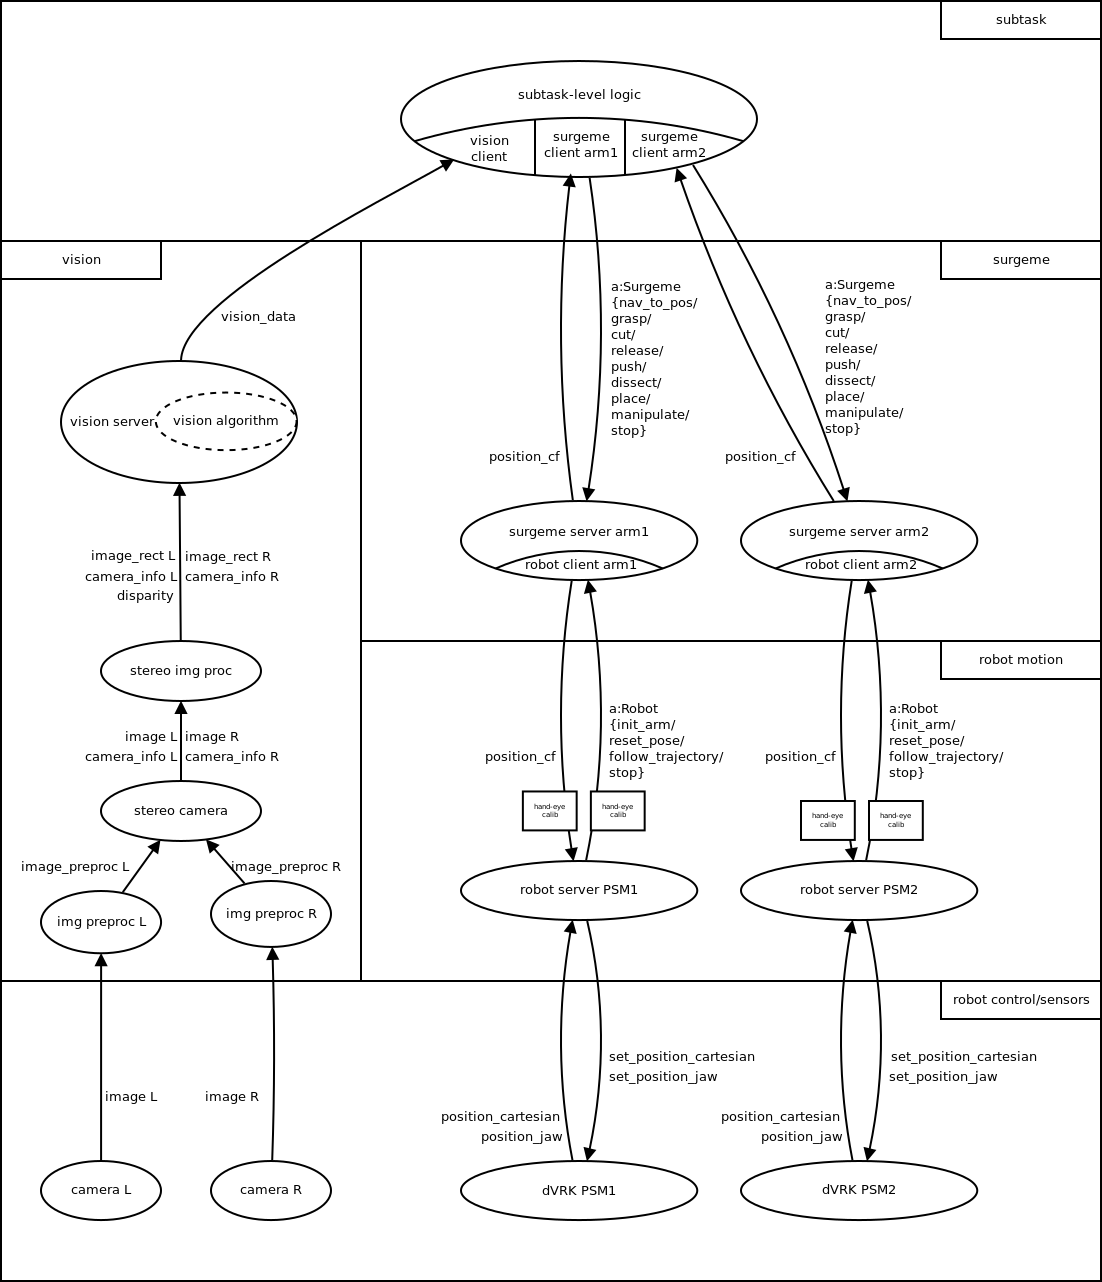
\includegraphics[width=14cm]{irobArch}
		\caption{A SAF sematikus működése, felépítése \cite{Abc-irobotics2020May} }
	\end{center}
\end{figure}
A \ref{fig:irob_web} ábrán láthatjuk a modul tervezett felépítését.
\begin{figure}[H]
	\centering
	\label{fig:irob_web}
	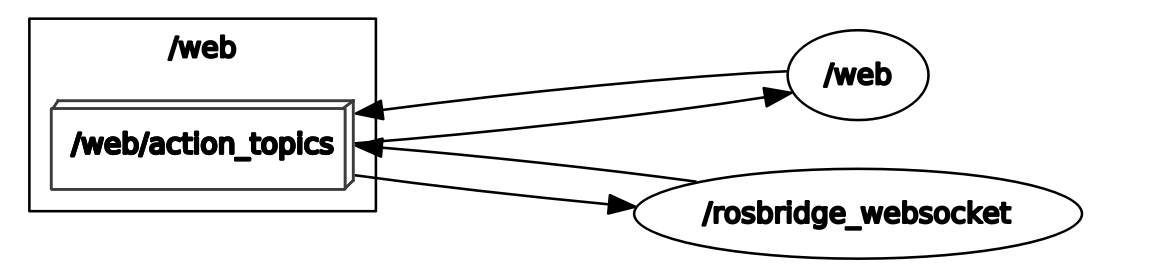
\includegraphics[width=14cm]{irob_web}
	\caption{ROS web node ki/be meneteli csatlakozásai}
\end{figure}


\subsubsection{Da Vinci WebShocket szerviz modul}
A modul működéséhez szorosan kapcsolódó programkönyvtár.
\paragraph{Standard ROS JavaScript könyvtár}
\label{roslibjs}
A Standard ROS JavaScript könyvtár továbbiakban roslibjs a Robot Web Tools része \cite{toris2015robot}.  Alap JavaScript könyvtár, ami a ROS környezettel való böngészőből történő interakció kialakítására készítettek. A Robot Web Tools olyan eszközök fejlesztésének gyűjteménye melyek célkitűzése a ROS rendszer böngészőből történő használatához készítenek, napjainkban is folyamatosan egyre több funkciót lehetséges elérni benne. A könyvtár két részből áll. Biztosít egy JavaScript könyvtárat melyen keresztül kéréseket tudunk megfogalmazni a ROS szerver számára nevezzük ezt most JavaScript könyvtárnak. A Robot Web Tools legfontosabb része a \textit{rosbridge} protokoll, ami a kiadott kérések fogadására van. A \textit{rosbridge\_server} egy ROS szolgáltatás amit el kell indítani, hogy továbbítsa a kéréseinket megfelelő ROS modul számára.

Ennek egy kiegészítő modul mely a konkrét csatlakozást teszi lehetővé a böngésző számára a ROS környezethez, ezt a modult nem nekem kell készítenem, csak használom a ROS környezet által nyújtott lehetőségeket.

\chapter{Megvalósítás}
\section{Da Vinci vizuális programozás összefoglaló}
A ROS modulok használata jelenleg Ubuntu 16.04-es verzióval van tesztelve. A Web modulokat én a mindenkori legfrissebb Manjaro Linux alól tesztelem, de elvi szinten bármilyen disztribúció alkalmas ezek használatra, a megfelelő függőségek feltelítése után. Az Ubuntu 16.04-et javaslom virtualizált környezetben futtatni.
Az alkalmazás szimulációval történő  da Vinci programozás használathoz a következőket kell tenni. A SAF keretrendszer leírásának megfelelően  el kell indítani egy dVRK PSM kar szimulációt \cite{irobotics2020May}. Majd egy SAF ''dummy`` objektumot kell elhelyezni a szimulációban. A szimulált kar állapotát ''home`` pozíció kell hozni. ''Dummy vision`` elindítás is szükséges. Következő szükséges lépés továbbra is a leírásának megfelelően irob\_robot szolgáltatás majd surgeme\_server szolgáltatás elindítása. A leírástól eltérve kell folyatni. Ez után a web\_actions modul futtatása szükséges. Következő lépésként pedig a '' rosbridge\_websocket`` futtatása szükséges. Ezek után meg vagyunk ROS oldalról. A következőkben az NodeJS szerver modul leírásának megfelelő utasítások futtatása szükséges \cite{aaronrancsik2020May}. Amennyiben ezzel is megvagyunk az alkalmazás localhost hálózton elindította szolgáltatásait. Melyet modern böngészők segítségivel el lehet érni.
\chapter*{Irodalomjegyzék}
\addcontentsline{toc}{chapter}{Irodalomjegyzék}  
\printbibliography[heading=none]
\newpage
\listoffigures
\addcontentsline{toc}{chapter}{Ábrák jegyzéke}


\end{document}